\documentclass[10pt]{article}
\usepackage[a4paper,margin=2.1cm]{geometry}
\usepackage[table]{xcolor}
\usepackage{booktabs}
\usepackage{tabularx}
\usepackage{pgfplots}
\pgfplotsset{compat=1.17}
\usepackage{sourcesanspro}
\pagestyle{empty}
\setlength{\parindent}{0pt}
\setlength{\parskip}{0.6em}

\definecolor{accent}{HTML}{20639B}
\definecolor{teal}{HTML}{3CAEA3}
\definecolor{inkgray}{HTML}{555555}

% KPI tile: \kpi{value}{label}{delta}
\newcommand{\kpi}[3]{%
  \colorbox{accent!8}{\begin{minipage}[t][1.9cm]{0.215\textwidth}
    \vspace{6pt}\centering
    {\Large\bfseries\color{accent}#1}\\[3pt]
    {\scriptsize\color{inkgray}#2}\\[3pt]
    {\small\bfseries\color{teal}#3}
    \vspace{4pt}
  \end{minipage}}}

\begin{document}

{\LARGE\bfseries\color{accent}Meridian Analytics}\hfill
{\large\bfseries Quarterly Business Report}

\vspace{2pt}
{\color{inkgray}\small Q2 2026 (April to June) \quad\textbullet\quad
Prepared for the board of directors \quad\textbullet\quad July 21, 2026}

\vspace{6pt}
{\color{accent}\rule{\linewidth}{2pt}}

\vspace{12pt}
{\large\bfseries\color{accent}Key performance indicators}

\vspace{6pt}
\kpi{\$1.72M}{QUARTERLY REVENUE}{+14\% YoY}\hfill
\kpi{84}{RECURRING CLIENTS}{+6 net new}\hfill
\kpi{118\%}{NET REVENUE RETENTION}{+3 pts QoQ}\hfill
\kpi{78.4\%}{GROSS MARGIN}{+0.8 pts QoQ}

\vspace{14pt}
{\large\bfseries\color{accent}Revenue by segment}

\vspace{4pt}
\begin{center}
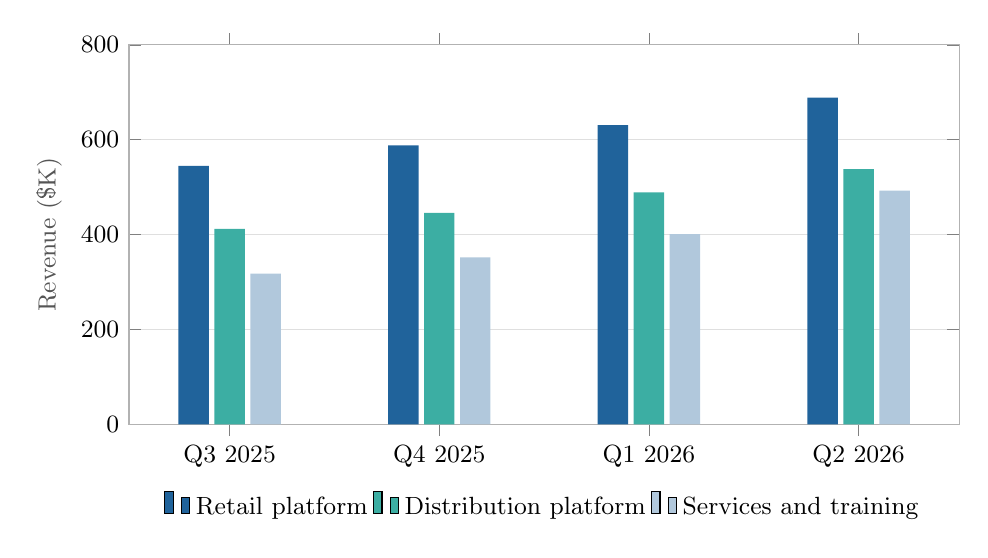
\begin{tikzpicture}
\begin{axis}[
  ybar,
  width=\textwidth,
  height=6.4cm,
  bar width=11pt,
  ymin=0, ymax=800,
  ylabel={Revenue (\$K)},
  ylabel style={font=\small, color=inkgray},
  symbolic x coords={Q3 2025, Q4 2025, Q1 2026, Q2 2026},
  xtick=data,
  tick label style={font=\small},
  ymajorgrids,
  grid style={gray!25},
  axis line style={gray!60},
  legend style={font=\small, draw=none, fill=none,
                at={(0.5,-0.16)}, anchor=north, legend columns=-1},
  enlarge x limits=0.16,
]
\addplot[fill=accent,  draw=none] coordinates
  {(Q3 2025,545) (Q4 2025,588) (Q1 2026,631) (Q2 2026,689)};
\addplot[fill=teal,    draw=none] coordinates
  {(Q3 2025,412) (Q4 2025,446) (Q1 2026,489) (Q2 2026,538)};
\addplot[fill=accent!35, draw=none] coordinates
  {(Q3 2025,318) (Q4 2025,352) (Q1 2026,401) (Q2 2026,493)};
\legend{Retail platform, Distribution platform, Services and training}
\end{axis}
\end{tikzpicture}
\end{center}

\vspace{6pt}
{\large\bfseries\color{accent}Highlights and outlook}

Revenue reached \$1.72M, ahead of the \$1.65M plan, driven by six net new
mid-market retail logos and the strongest services quarter to date.
Services growth reflects onboarding for the March cohort and is expected
to normalize in Q3 as those clients move to steady state.

\rowcolors{2}{accent!6}{white}
\begin{tabularx}{\textwidth}{@{}Xrrr@{}}
  \toprule
  \rowcolor{white}
  {\bfseries Measure} & {\bfseries Plan} & {\bfseries Actual} & {\bfseries Variance}\\
  \midrule
  New bookings (ACV) & \$620K & \$707K & +14.0\%\\
  Churned ACV & \$95K & \$71K & $-$25.3\%\\
  Operating expense & \$1.31M & \$1.28M & $-$2.3\%\\
  Cash at quarter end & \$4.9M & \$5.3M & +8.2\%\\
  \bottomrule
\end{tabularx}

\vspace{4pt}
{\color{inkgray}\small Outlook: Q3 revenue is planned at \$1.81M. The
principal risk is the Frankfurt region timeline, which gates roughly
\$180K of committed EU bookings.}

\end{document}
